\documentclass[a4paper]{article}
\usepackage[T1]{fontenc}
\usepackage[utf8]{inputenc}
\usepackage[french]{babel}
\usepackage{url}
\usepackage{amsfonts}
\usepackage{amsmath}
\usepackage{amsthm}
\usepackage{hyperref}
\usepackage{graphicx}
%\usepackage{titling}
%\usepackage{tocloft}
\usepackage{float}

%\setlength{\droptitle}{-10em}
%\setlength{\cftsecnumwidth}{7mm}

\renewcommand{\thesection}{\Roman{section}}
\renewcommand{\thesubsection}{\thesection.\arabic{subsection}}

\newcommand{\cont}{\mathcal{C}^0}
\newcommand{\cun}{\mathcal{C}^1}
\newcommand{\cinf}{\mathcal{C}^\infty}
\newcommand{\R}{\mathbb{R}}
\newcommand{\N}{\mathbb{N}}
\newcommand{\oB}{\overline{B}}

\newtheorem{thm}{Théorème}
\newtheorem*{thm*}{Théorème}
\newtheorem{lemm}{Lemme}
\theoremstyle{definition}
\newtheorem{defn}{Définition}

\begin{document}
\title{Annexes}
\author{Farid Arthaud}
\maketitle
\tableofcontents

\section{Bibliographie}
\begin{enumerate}
	\item \textit{Stabilité structurelle et morphogenèse}, René \textsc{Thom} (\textit{1974})
	\item \textit{Catastrophes et bifuractions}, Michel \textsc{De Mazure} (\textit{1989})
	\item \textit{Catastrophe theory and its applications}, Tim \textsc{Poston}, Ian \textsc{Stewart} (\textit{1978})
\end{enumerate}

\section{Intersections transverses}
\begin{figure}[H]
	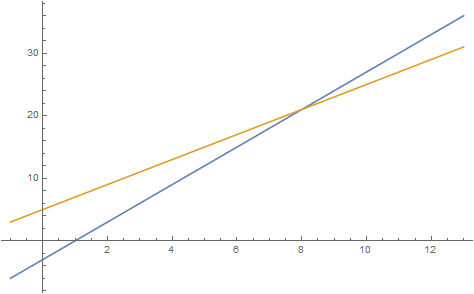
\includegraphics[width=10cm,keepaspectratio]{images/2DTransverse.png}
	\caption{Intersection transverse dans $\R^2$}
\end{figure}
\begin{figure}[H]
	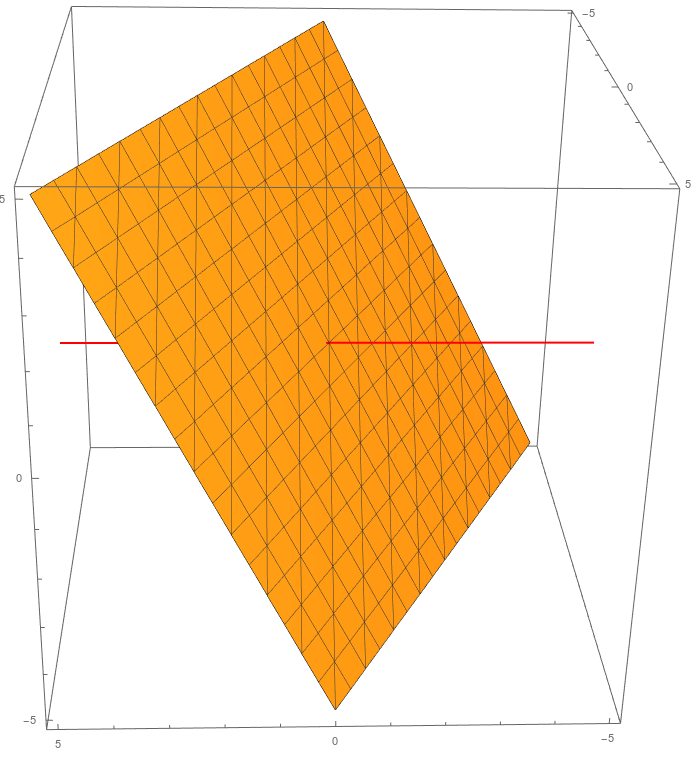
\includegraphics[width=8cm,keepaspectratio]{images/3D_trans.png}
	\caption{Intersection transverse dans $\R^3$}
\end{figure}
\begin{figure}[H]
	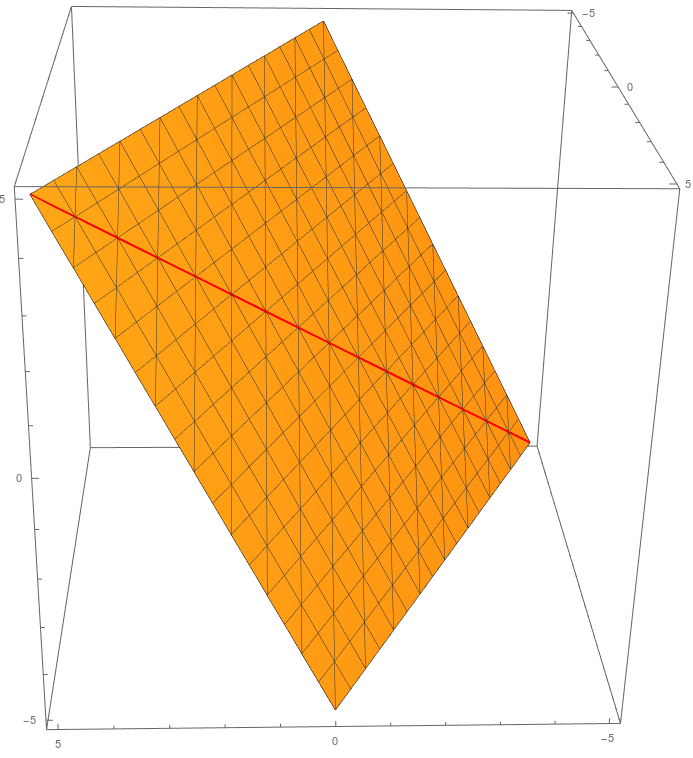
\includegraphics[width=8cm,keepaspectratio]{images/3D_non_trans.png}
	\caption{Intersection non transverse dans $\R^3$}
\end{figure}

\section{Inversion locale, fonctions implicites}

\subsection{Théorème d'inversion locale}

\setcounter{thm}{3}
\begin{thm}[d'inversion locale]
	Si $f\in\cinf(U,\R^m)$, et que $df_a$ est bijective, alors f est un difféomorphisme local: elle est bijective d'un voisinage de $a$ vers un voisinage de $f(a)$, de réciproque $\cinf$.

	On en déduit qu'au voisinage de $a$, il existe un système de coordonnées locales telles que $f(x)=f(a)+x$, ou encore que $(a,f)$ est équivalent à $(0,Id)$.
\end{thm}
\begin{proof}[Démonstration (cas $\cun$)]
	On se ramène à un voisinage de 0 où $df_0=Id_E$ (et donc $E=\R^m$) en prenant pour fonction $df_a^{-1}(f(a+x)-f(a))$ que l'on notera dorénavant $f$.
	Pour $r$ assez petit fixé, on a $\forall x\in B_r(a), \| df_x-Id_E \| \leq \frac{1}{2}$.

	On pose, pour $y$ fixé de $B_{\frac{r}{2}}$, $h:x\mapsto x+y-f(x)$.
	On a, par les accroissements finis sur $B_r, \| h(x) - h(x')\|\leq\frac{\| x-x' \|}{2}$, donc h contractante.
	Elle est de plus à images dans $B_r$ (en prenant $x'=0$), donc y admet un unique point fixe: $y$ admet un antécédent unique par $f$ dans $B_r$.
	$f$ est donc bijective $f^{-1}(B_\frac{r}{2}) \cap B_r \to B_{\frac{r}{2}}$.

	Quant à la continuité de la réciproque, on a:
	$$\|x-x'\| \leq \|h(x)-h(x')\| + \|f(x)-f(x')\| \implies \|x-x'\| \leq 2\|f(x')-f(x)\|$$
	En l'appliquant à $f^{-1}(y)$ et $f^{-1}(y')$ on obtient $f^{-1}$ 2-lipschitzienne.

	Enfin, pour la différentiabilité, on choisit $k$ proche de 0 et on pose $h=f^{-1}(y+k)-f^{-1}(y)$.
	On peut écrire $df_x=Id_E-u$ et donc avoir $df_x^{-1}=\sum_{k\geq0} u^k$ qui donne $\|df_x^{-1}\| \leq 2$.

	On constate que $\|h\|\leq 2\|k\|)$, puis
	\begin{align*}\| f^{-1}(y+k)-f^{-1}(y)-(df_x)^{-1}(k) \| & = \|df_x^{-1}(f(x+h)-f(x)-df_x(h))\| \\ & \leq 2\| f(x+h)-f(x)-df_x(h) \| =o(h) \\ & = o(k)\end{align*}
\end{proof}

%\textit{Corollaire classique}: si $f\in\cinf$ est injective et $df_a$ est inversible, alors il existe un voisinage de $a$ dont l'image par $f$ est un ouvert, et $f$ est un difféomorphisme local.

\subsection{Théorème des fonctions implicites}

Soit $f\in\cinf(\R^n\times\R^m,\R^p)$ et on note $f_2(y) = f(x_0, y)$.
Si $df_{2,y_0}$ est difféomorphisme local (donc $f_2$ localement inversible), alors il existe une application $\phi_c$ telle que $f(x,\phi_c(x))=c$ sur un voisinage de $(x_0,y_0)$, et ce pour tout $c$ au voisinage de $f(x_0,y_0)$.

Cela signifie que $c$ admet un unique antécédent par $y\mapsto f(x,y)$ pour $x$ suffisament proche de $x_0$.

\bigskip

On notera que ces deux théorèmes restent valables sous des hypothèses moins fortes de régularité, et que ces hypothèses sont héritées par $\phi$ et $f^{-1}$ dans ces cas.
De plus, les démonstrations de chacun de ces théorèmes se déduisent facilement de l'énoncé de l'autre.

\section{Lemmes d'\textsc{Hadamard}, de \textsc{Morse}}

\subsection{Lemme d'\textsc{Hadamard}}
\begin{lemm}[d'\textsc{Hadamard}]
	Si $f$ est $\cinf$ et s'annule en $0$, alors il existe un voisinage de $0$ sur lequel $f$ peut s'écrire: $f(x)=x_1g_1(x)+...+x_ng_n(x)$ avec $g_i\in\cinf$ et $g_i(0) = \frac{\partial f}{\partial x_i}(0)$.
\end{lemm}
\begin{proof}
	On pose:
	$$g_i(x) = \int_0^1 \frac{\partial f}{\partial x_i}(tx)dt$$

	Le théorème de dérivation d'une intégrale à paramétre donne bien $g_i\in\cinf$ et on a évidemment $g_i(0) = \frac{\partial f}{\partial x_i}(0)$.
	De plus,
	$$x_1g_1(x)+...+x_ng_n(x)=\int_0^1 df_{tx}(x) dt = f(x)$$
\end{proof}

\subsection{Lemme de \textsc{Morse}}
\begin{lemm}[de \textsc{Morse}]
	Si $f\in\cinf(\R^n,\R)$ admet un point critique non dégénéré en $u$, alors il existe un voisinage de $u$ et un $\cinf$-difféomorphisme $y=(y_1,...,y_n)$ tel que:

	$$f=f(u)+y_1^2+...+y_l^2-y_{l+1}^2-...-y_n^2$$
\end{lemm}
\begin{proof}
	On montre par récurrence sur $r$ que $f$ s'écrit pour certaines coordonnées
	$$f(x)=\pm u_1^2 \pm...\pm u_{r-1}^2 + \sum_{i,j\geq r} u_iu_jH_{ij}(u)$$
	avec $H_{i,j}\in\cinf$.

	Le rang $r=1$ se déduit du \textit{lemme d'\textsc{Hadamard}}. On peut de plus supposer $H_{i,j}=H_{j,i}$ en moyennant les termes $i,j$ et $j,i$.
	On peut supposer $H_{rr}(0)\neq0$ par un changement de coordonnées, puisque $(H_{i,j}(0))_{i,j}$ est inversible donc $(H_{i,j}(x))_{i,j}$ est symétrique inversible par continuité.

	On pose alors $$u_r' =\sqrt{\mid H_{rr}\mid}\big(u_r+\sum_{i>r}u_i\frac{H_{ir}}{H_{rr}}\big)$$
	$(u_1,...,u_{r-1},u'_r,u_{r+1},...,u_n)$ sont bien des coordonnées locales selon le \textit{théorème d'inversion locale}, et donc il s'agit bien d'un changement de coordonnées.

	On réécrit alors $f$ comme précédemment mais en allant jusqua'au rang $u_r'$ au lieu de $u_{r-1}$ (attention, $(u_r')^2$ donne un reste à ajouter pour former de nouveaux $H_{ij}$).
\end{proof}

\section{Généricité et Théorème de \textsc{Baire}}
\begin{defn}
	Une propriété sur des éléments d'un espace topologique $E$ est dité \textbf{générique} si elle est vérifiée sur une intersection dénombrable d'ouverts denses.
\end{defn}

\begin{thm*}[de \textsc{Baire}]
	Dans un espace normé complet, une intersection dénombrable d'ouverts denses est dense.
\end{thm*}
\begin{proof}
	Soit $(O_n)_n$ une famille d'ouverts denses de $E$ un espace normé complet, et $V$ un ouvert quelconque.

	On construit une suite de boules ouvertes $(B_n)_n$ de rayons au plus $2^{-n}$ vérifiant $\forall n\geq0, \oB_{n+1} \subseteq O_{n+1}\cap B_n$.

	Pour $B_0$, on choisit une boule dans $O_0 \cap V$ ouvert non vide, de rayon au plus $1$ et de fermeture incluse dans $O_0 \cap V$ (quitte à réduire le rayon).
	Ensuite, si les $n\geq1$ premières boules sont construites, $O_{n} \cap B_n$ est un ouvert non vide par densité, dans lequel on peut donc choisir une boule $B_{n+1}$ vérifiant les propriétés précédentes.

	Par complétude, on a $\cap_{n\geq0} B_n \neq \emptyset$: toute suite de points pris dans chaque boule constitue une suite de \textsc{Cauchy}.
	Un point de cette intersection est dans l'intersection des $O_n$ par une récurrence immédiate, et dans $B_0 \subset V$.
\end{proof}

\section{Surfaces dans $\R^3$}
\subsection{Points-plis et points-fronce}
\begin{figure}[H]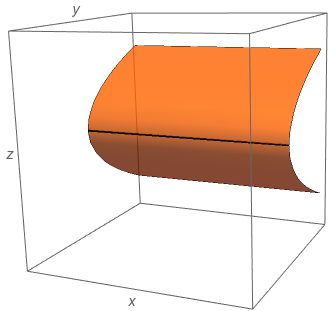
\includegraphics[width=8cm, keepaspectratio]{images/fold_front.png}\caption{Point-pli avec les contours apparents en noir}\end{figure}
\begin{figure}[H]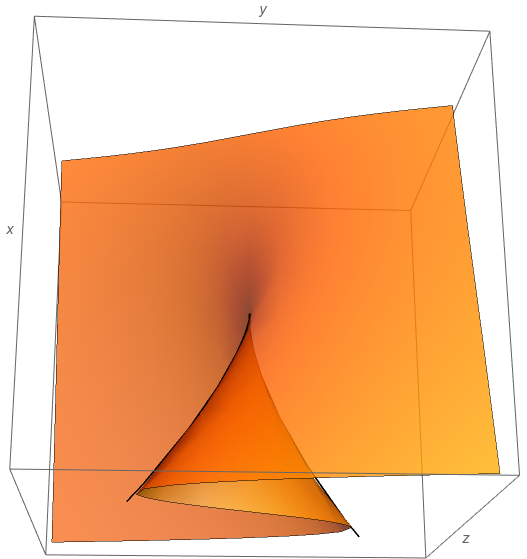
\includegraphics[width=8cm, keepaspectratio]{images/cusp_side.png}\caption{Point-fronce avec les countours apparents en noir}\end{figure}

Dans cette dernière illustration, la courbe de contour apparents (en noir) correspond à des points-plis excepté le point à l'extrémité, ou le point de rebroussement est en fait un point-fronce.

Ceci illustre l'énoncé du théorème suivant, puisque les points-plis forment une courbe le long d'une surface, et le point-fronce est isolé le long de cette courbe.

\subsection{Théorème}
\setcounter{thm}{6}
\begin{thm}
	Pour $f$ générique:
	\begin{enumerate}
		\item $\{f=0\}$ est une sous-variété de dimension deux (ou une \textbf{surface})
		\item Son contour apparent $\{f=0\}\cap \{\frac{\partial f}{\partial z}=0\}$ est une sous-variété de dimension un (ou une \textbf{courbe})
		\item Tous les points critiques sont des points-plis ou points-fronces, et les points-fronces sont isolés
	\end{enumerate}
\end{thm}
\begin{proof}[Démonstration (deux premiers points)]
	Il est clair que $\{f=0\}$, $\{f=\frac{\partial f}{\partial z}=0\}$ et $\{f=\frac{\partial f}{\partial z}=\frac{\partial^2 f}{\partial z^2}=0\}$ sont des sous-variétés de l'espace des germes $J^2(\R^3,\R)$ de codimensions $1$, $2$ et $3$: on applique donc le théorème de transversalité de \textsc{Thom} ainsi que celui sur la dimension d'une image réciproque pour obtenir les deux premiers points.

	On obtient donc que $\{f=0\}$ est une variété de codimension $1$ (une surface, éventuellement vide), $\{f=\}=\frac{\partial f}{\partial z}=0\}$ est une sous-variété de codimension $2$ (une courbe, éventuellement vide) et que $\{f=\frac{\partial f}{\partial z}=\frac{\partial^2 f}{\partial z^2}=0\}$ est une sous-variété de codimension $0$, soit un ensemble discret de points de $\R^3$.

	En réitérant ceci avec les germes troisièmes, on constate que les points où les trois premières dérivées de $z \mapsto f(x,y,z)$ s'annulent est vide.

	Quant à la réecriture au voisinage d'un point critique, il faut distinguer les cas selon $\frac{\partial^2 f}{\partial z^2}$ nul ou non, et utiliser la remarque précédente ainsi que le théorème de décomposition.
\end{proof}

\end{document}

%%%%%%%%%%%%%%%%%%%%%%%%%%%%%%%%%%
\section{Classification des formes quadratiques}

\subsection{Généralités}

Est appelée forme quadratique toute forme $f:\R^n\to\R$ de type $$f(x_1,...,x_n)=\sum_{1\leq i,j\leq n}\lambda_{ij}x_ix_j$$

On associe alors à $f$ une matrice diagonale symmétrique $\Lambda$. Or toute matrice symétrique est diagonalisable en une matrice orthogonale: $\exists M \in \mathcal{O}(\R) / \Lambda = M^T\cdot D\cdot M$. Ceci permet donc d'écrire $f(X) = (M\cdot X)^T\cdot D\cdot (M^{-1}\cdot X)$.

\textit{Preuve}: On se ramène au cas où $\lambda_{11} \neq 0$ soit par échange de lignes si un autre terme diagonal est non nul, soit en posant $y_i=\frac{1}{2}(x_i+x_j)$ et $y_j=\frac{1}{2}(x_i-x_j)$ si $\lambda_{ij}\neq 0$. On factorise ensuite l'expression de $f$ par $\lambda_{11}$, et on constate que si l'on note $\mu_{ij}=\frac{\lambda_{ij}}{\lambda_{11}}$, alors les termes en $x_1$ sont exactement:
$$x_1^2+2\sum_{j=2}^n \mu_{1j}x_1x_j=\big(x_1+\sum_{j=2}^n \mu_{1j}x_j\big)^2-\big(\sum_{j=2}^n \mu_{1j}x_j\big)^2$$

En posant $y_1$ égal au premier terme de cette différence, on a une expression du type $f(y)=\lambda_{11}y_1+$ un reste quadratique en $n-1$ variables. Par récurrence, on obtient bien une matrice diagonale.

Par changement de base, on peut donc écrire $f(X) = X\cdot D\cdot X^T$ avec $D$ diagonale. En normalisant, on peut considérer $D$ diagonale à coefficients dans $\{-1,0,1\}$. Enfin, en changeant l'ordre des vecteurs de la base on se ramène au cas où f est de la forme:
$$f(x_1,...,x_n)=x_1^2+x_2^2+...+x_k^2-x_{k+1}^2-...-x_s^2$$

On constate par ailleurs que $s=rg(\Lambda)=rg(f)$ et $sgn(\Lambda)=k-(s-k)=2k-s$. En général, il faut $\frac{n(n+1)}{2}$ coefficients pour décrire une telle forme, mais on se ramène ici à $n$ nombres (1, -1 ou 0) modulo une base.

\subsection{Cas de $n=2$}

On a alors $f(x,y)=ax^2+2bxy+cy^2$, et $0\leq rg(f)\leq 2$ ainsi que $0\leq k\leq rg(f)$. Comme vu ci-dessus, deux formes quadratiques de rang et signature égaux sont équivalentes à changement de base près. On peut donc catégoriser en $1+2+3=6$ classes les formes quadratiques:

\begin{itemize}
\item  $Q_{2,2}$: $x^2+y^2$
\item  $Q_{2,0}$: $x^2-y^2$
\item  $Q_{2,-2}$: $-x^2-y^2$
\item  $Q_{1,1}$: $x^2$
\item  $Q_{1,-1}$: $-x^2$
\item  $Q_{0,0}$: $0$

\end{itemize}

\section{Classification des formes cubiques ($n=2$)}

\subsection{Noyaux de formes cubiques}

Une forme cubique de deux variables est une application $$f: (x,y) \mapsto \alpha x^3+\beta x^2y+\gamma xy^2+\delta y^3$$

Ces applications se divisent en cinq catégories en fonction de $(\alpha,\beta,\gamma,\delta)$. Cherchons une classification à partir du noyau de $f$. Ce noyau est stable par $\cdot$ la loi de composition externe, et peut donc être vu comme un ensemble de droites passant par l'origine dans $\R^2$.

En cherchant l'intersection de ces droites avec $x=1$ (en prenant garde à la droite $x=0$), on cherche à résoudre $\alpha+\beta y+\gamma y^3=0$. Si au moins un coefficient est non nul, cette équation admet au plus 3 solutions réelles (et un nombre pair de racines complexes), donc on distingue cinq catégories de noyaux:

\begin{itemize}
\item  $C_{3,0}$: Trois droites distinctes
\item  $C_{1,0}$: Une droite unique
\item  $C_{3,2}$: Trois droites dont deux coïncidantes (racine double)
\item  $C_{3,3}$: Trois droites coïncidantes (racine triple)
\item  $C_{\infty,0}$: Le plan en entier (cas où $(\alpha,\beta,\gamma,\delta)=(0,0,0,0)$)

\end{itemize}

Ceci découle du fait que si la droite $x=0$ est dans le noyau, alors $\delta=0$ et on se retrouve avec un polynôme du second degré en $y$, et donc bien au plus trois droites.

Ces catégories en sont bien, car aucun changement de coordonnées ne fera varier le `nombre de droites du noyau' (à voir en termes de déformation du plan, les droites coïncidantes coïncident toujours et celles distinctes restent distinctes).

\subsection{Equivalence des classes}

Deux fonctions appartenant à la même catégorie de noyau ont la même expression à changement de coordonées linéaire près. Une analyse de chaque cas donne:

\begin{itemize}
\item  $C_{3,0}$: $f(x,y)=x^2y-y^3$
\item  $C_{1,0}$: $f(x,y)=x^2y+y^3$
\item  $C_{3,2}$: $f(x,y)=x^2y$
\item  $C_{3,3}$: $f(x,y)=x^3$
\item  $C_{\infty,0}$: $f=0$

\end{itemize}
\begin{proof}
	Un changement de base dans le premier cas permet de déformer le plan de manière à obtenir un carré: les trois droites correspondent aux abscisses, ordonées et l'identité. Alors, $f$ est divisible par $xy(x-y)$, et à changement de base supplémentaire ($(x',y')=\frac{1}{2}((x+y),(x-y))$) on obtient $f(x,y)=x^2y-y^3$.

	Dans les autres cas, on considère une des droites, d'expression $lx+my=0$. $f$ peut être factorisée par cette expression, et l'on obtient une de trois catégories de formes quadratiques: $Q_{1,1}$ et $Q_{1,-1}$ ainsi que $Q_{2,2}$ et $Q_{2,-2}$ peuvent être fusionées, car le signe peut être compensé par le changement $(x,y)=-(x,y)$.

	Par changement de coordonées, on est donc ramené à l'un des cas: $(Lx+My)(x^2-y^2)$ ou $(Lx+My)x^2$ ou $(Lx+My)(x^2+y^2)$. Le premier de ces cas nous ramène soit aux trois droites, soit au second cas (selon si $(Lx+My)$ est multiple de $(x-y)$ ou $(x+y)$ ou non). Le second cas mène soit à $x^3$ (si $M=0$) ou $xy^2$. Le troisième est $(x^2+y^2)y$ (soit $LM=0$, ou on procède à une \textit{rotation des axes} $(x',y')=\frac{1}{\sqrt{L^2+M^2}}(Ly-Mx,Lx+My)$).
\end{proof}

\section{Théorème de décomposition}
\begin{thm}[de décomposition]
	Si f admet 0 pour point critique et $H(f)_0$ est de rang $r$, alors $f$ est équivalente (au sens défini ci-dessus) au voisinage de 0 à une fonction de la forme:

	$$g(x)= x_1^2+x_2^2+ ...+x_p^2-x_{p+1}^2 -...- x_r^2 + h(x_{r+1},...,x_n)$$
\end{thm}
\begin{proof}
On suppose $H(f)_0$ de rang 1.
Via un changement de base, on peut supposer $\frac{\partial f}{\partial x}(0,0) \neq 0$. On applique alors le \textit{théorème des fonctions implicites} à $\frac{\partial f}{\partial x}$ pour obtenir $\varphi$ telle que $\frac{\partial f}{\partial x}(\varphi(y), y)=0$ pour tout $y$ proche de 0.

Le difféomorphisme local $\Phi: (x,y) \mapsto (x+\varphi(y), y)$ permet de poser $F(u,v) = f\circ\Phi(u,v)$ vérifiant $\frac{\partial F}{\partial u}=\frac{\partial f}{\partial x}$ et $\frac{\partial F}{\partial u}=0 \iff u=0$.

Le \textit{lemme d'\textsc{Hadamard}} nous permet alors d'écrire $F(u,v)=\alpha(v)+u^2\beta(u, v)$ (car ?)
\end{proof}
\begin{proof}
	On travaille dans $\cinf$.
	Alors $H(f)_0$ peut être mise sous la forme d'un bloc diagonal de 1 et de -1 de format $r\times r$ par un changement de base (selon le \textit{lemme de Morse}) et des 0 partout ailleurs.
	On applique le \textit{théorème des fonctions implicites} en (0,0) (d'image 0) à
	$$(x_1,...,x_r),(x_{r+1},...,x_n)\mapsto \big(\frac{\partial f}{\partial x_1}(x), ..., \frac{\partial f}{\partial x_r}(x)\big)$$

	On obtient alors $g$ telle que $(g(x_{r+1},...,x_n),x_{r+1},...,x_{r})$ soit l'ensemble des points pour lesquels l'image de la fonction précendente soit nulle. Notons alors $F: x\mapsto ((x_1,...,x_r)+g(x_{r+1},...,x_n),x_{r+1},...,x_{r})$ qui correspond à $f$ à un changement de coordonées près, puisque

	Tout a était fait afin que F
\end{proof}
